\documentclass[12pt]{article}

% PACKAGE USING
\usepackage[top = 1in, bottom = 1in, left = 0.75in, right = 0.75in]{geometry}
\usepackage{amsmath, amssymb, amsthm, amsfonts}
\usepackage{xcolor}
\usepackage{graphicx, subcaption}
\usepackage{url, hyperref}
\hypersetup{
    colorlinks = true,
    urlcolor = blue,
    citecolor = red
}
\usepackage{biblatex}
\addbibresource{references.bib}


\newcommand{\Q}{\mathbb{Q}}
\newcommand{\E}{\mathbb{E}}
\newcommand{\R}{\mathbb{R}}



\begin{document}

\begin{titlepage}
    \begin{center}
        \vspace*{5cm}
 
        \Huge{\textbf{Research Reading and Critical Assessment Assignment}}
 
        \vspace{0.5cm}
        \large{of the paper titled ``Detecting and repairing arbitrage in traded option prices''}\\
        \large{by}\\
        \large{Samuel N. Cohen, Christoph Reisinger and Sheng Wang}
             
        \vspace{1.5cm}
 
        \large{\textit{Prepared by,}}\\
        \large{\textbf{Subhrajyoty Roy}}\\
        \large{\textbf{MB1911}}
 
        \vspace{2cm}
             
        \textit{Assignment for Quantitative Finance course\\
        as a part of Master of Statistics curriculum}\\
        \vspace{0.5cm}
        \textbf{Session: } 2020-21\\
        Indian Statistical Institute, Kolkata

        \vfill
        
        \begin{flushright}
            \normalsize{\today}            
        \end{flushright}
    \end{center}
\end{titlepage}


\section{Introduction}

Absence of arbitrage in a financial market is a very crucial assumption in almost all of the theoretical developements~\cite{hull2003options,pliska1997introduction,ross2011elementary}. While it is theoretically meaningless to have a model that allows the potential to make risk-free profits, the financial market data which one has to analyze for day-to-day decision making may suggest the existence of arbitrage opportunity. Even when there are no instrumental or operational errors in data recording, such arbitrage opportunity may actually be implicitly present in the market due to the following reasons:

\begin{enumerate}
    \item Imperfect information between the players of the financial market.
    \item Existence of transaction costs.
    \item Freedom of deviating from a self-financing strategy.
    \item Freedom of intra-day trading of financial contracts.
    \item Existence of unofficial or illegal financial markets.
\end{enumerate}

Different techniques such as smoothing~\cite{ait2003nonparametric,fengler2009arbitrage,fengler2015semi} and data truncation and filtering~\cite{ivanovas2014option} exist to detect and remove arbitrage from price data. However, since filtering usually truncates the data and smoothing usually changes all of the data to match an underlying nonparametric model, both results in information loss. In contrast, the paper by Cohen, Reisinger and Wang~\cite{cohen2020detecting} performs detection of arbitrage and repair the data as necessary without any information loss.

\section{Discussion on the paper}

The idea presented in the paper is to construct different constraints starting from a no-arbitrage market. Once such constraints are created, the deviations from these constraints are computed in the light of available pricing data, and a linear programming problem is formed to minimize the $L_1$ norm of the errors. 

It starts by assuming $n$ vanilla call options with maturity dates being in the set $\{ T_1, \dots T_m \}$ (arranged in increasing order), where at each maturity date $T_i$, there are $n_i$ options available with strike prices $0 < K_1^i < \dots < K_{n_i}^i$. The $(i,j)$-th option has a price $C_j^i$ at time $0$, and has a payoff $(S_{T_i} - K_j^i)^+$. \textbf{In this setting, the paper makes a crucial assumption that all the options are made only on a single risky asset, and no arbitrage opportunity can be extracted with a call option on one stock and put option with another.}

Next, it assumes a \textbf{frictionless market, where no transaction costs are present}. The authors circumvent this by indicating that single-price data are not executable prices in the market, but are designed to be benchmark prices for tradable assets, which are useful inputs to various models. \textbf{However, such an argument then advises against using the method in day-to-day trading price determination and decision making, which is one of the most significant area to detect arbitrage.} To account for discounting, it is assumed that zero-coupon bonds and forward contracts on the risky asset, with the same expiries as the options, are traded in the market, and their prices are \textbf{known without any error}. \textbf{However, in practice, the interest rates on the bonds may be flexible and change if the maturity period is long}. In other words, the discounting factor $D_i = D(T_i)$ and forward prices $F_i = F(T_i) = S_0/(D(T_i)\Gamma(T_i))$ (where $\Gamma(T_i)$ is the expected number of risky asset at time $T_i$ for a unit-value self financing strategy) are known along the price data. 

The Fundamental Theorem of Asset Pricing establishes an equivalence between no-arbitrage and existence of an equivalent martingale measure (note that the measure may not be unique for incomplete market). Under such an equivalent martingale measure $\Q$ we have 

\begin{equation}
    \dfrac{C_j^i / D_i}{F_i} = \E_{\Q} \left[ \left( \dfrac{S_{T_i}}{F_i}  - \dfrac{K_j^i}{F_i} \right)^+  \mid \mathcal{F}_0 \right] 
    \label{eqn:ctk}
\end{equation}

\noindent where $\mathcal{F}_0 = \{ \Omega, \phi \}$, the trivial filtration. The Eq.~\eqref{eqn:ctk} can be interpreted as, the expected payoff that one can gain from buying the $(i,j)$-th call option that time $0$, should be equal to the riskless payoff by putting the amount equal to the price of the option in savings, in relative to a forward contract. Equipped with this, one defines the normalized call function (which is used for pricing of the options under no-arbitrage), 

\begin{equation*}
    c(T, K) = \E_{\Q} \left[ \dfrac{\left( S_T - K \right)^+}{F(T)} \mid \mathcal{F}_0 \right]
\end{equation*}

\begin{figure}[ht]
    \centering
    \begin{subfigure}[b]{0.49\linewidth}
        \centering
        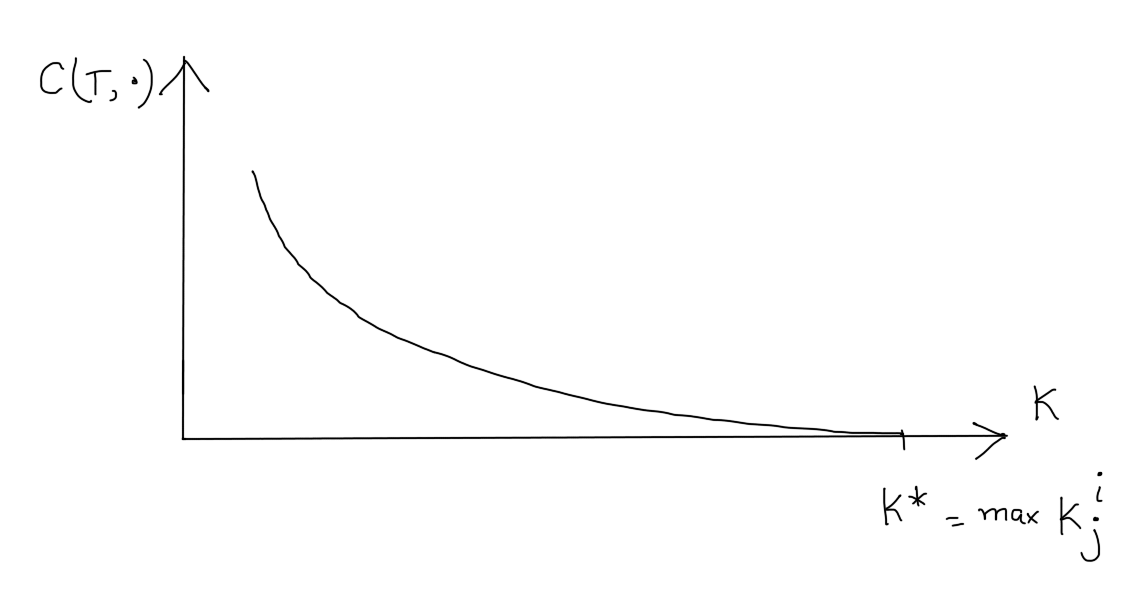
\includegraphics[width = \linewidth]{ctk.png}
        \caption{Typical form of a call function}
        \label{fig:call-function}
    \end{subfigure}
    \begin{subfigure}[b]{0.49\linewidth}
        \centering
        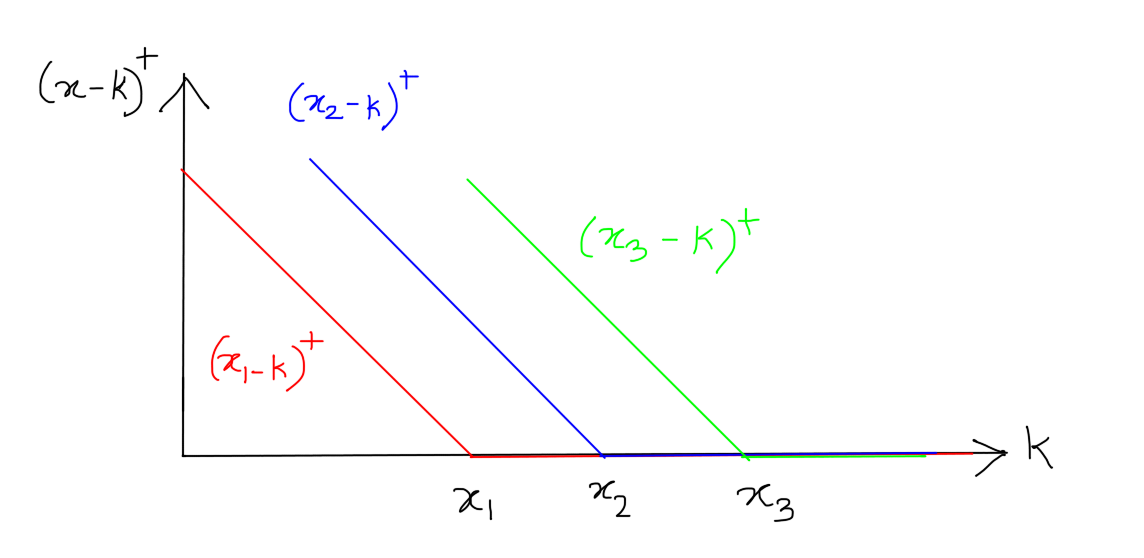
\includegraphics[width = \linewidth]{xkplus.png}
        \caption{Typical form of hinge functions (basis of the call functions)}
        \label{fig:hinge-function}
    \end{subfigure}
\end{figure}

A very desirable property of this call function is that for fixed $T$, $c(T, \cdot)$ should be a decreasing and convex function. Figure~\ref{fig:call-function} depicts a typical example of such call function for fixed $T$. However, this simple property also turns out to be sufficient to imply existence of such call function~\cite{breeden1978prices} and thereby a marginal martingale measure $\Q_T = \E_{\Q} \left[ \cdot \mid \mathcal{F}_T \right]$. Then, Kellerer's Theorem~\cite{kellerer1972markov} claims that such marginal martingale measure exists if and only if these $\Q_T$'s are in non-decreasing convex order, i.e. 

$$
\forall T_1 > T_2, \ \int_{\R} \phi d\Q_{T_1} \geq \int_{\R} \phi d\Q_{T_2} \qquad \text{for all convex functions } \phi
$$

\noindent To ensure this, note that the set of hinge functions $\{ (x - k)^+ : x \in \R \}$ (as a function of $k$) provides a basis for such non-decreasing call functions. In other words, for any call function $c(T, \cdot)$, there exists $\beta_{x_i}$'s such that, 

$$
\sup_{k \in \R} \left\vert c(T, k) - \sum_{i = 1}^{n} \beta_{x_i} (x_i - k)^+ \right\vert \xrightarrow{n \rightarrow \infty} 0
$$


\noindent Now, $c(T, k)$'s are available from the pricing data for $T = T_1, \dots T_m$ and $K = K_1^1, \dots K_{n_m}^m$. Therefore, the only required $\beta_{x_i}$'s that we can obtain from the price data are simply 

$$
\beta(i_1, j_1; i_2, j_2) = \dfrac{(c_{j_1}^{i_1} - c_{j_2}^{i_2})}{k_{j_1}^{i_1} - k_{j_2}^{i_2}}, \ \text{where, } c_{j}^i = \dfrac{C_j^i / D_i}{F_i} \text{ and } k_j^i = \dfrac{K_j^i}{F_i}
$$

\noindent Based on these $\beta(i_1, j_1; i_2, j_2)$ coefficients, several test strategies are formed such as vertical spread, calendar spread, vertical butterfly etc (see Table 1 of~\cite{cohen2020detecting}). Then, it is shown that no arbitrage opportunity present in these finite set of test strategies are enough to ensure no arbitrage in the original setup. \textbf{If any of the call option prices is missing, then the corresponding $\beta$ coefficient cannot be formed, hence some of the arbitrage opportunities cannot be verified}.

Final detection and repairing of the price data are performed by replacing the normalized prices $\boldsymbol{c}$ by $(\boldsymbol{c} + \boldsymbol{\epsilon})$, and then satisfying the finite set of static arbitrage conditions $\boldsymbol{A}(\boldsymbol{c} + \boldsymbol{\epsilon}) \geq \boldsymbol{b}$. Hence, the LP problem which is to be solved is given by 

$$
\min_{\boldsymbol{\epsilon}} \Vert \boldsymbol{\epsilon} \Vert_{L_1} \ \text{ such that } \boldsymbol{A}(\boldsymbol{c} + \boldsymbol{\epsilon}) \geq \boldsymbol{b}
$$

\noindent and minimization of $L_1$ norm sets most of the errors equal to $0$, and only retain the significant ones (similar to the idea of Lasso). If the bid-ask spread is known, the objective function can be re-expressed as $\sum_j f_j(\epsilon_j)$, where $f_j$'s are functions which give lower cost to errors within bid-ask bounds, but higher cost outside these bounds. Figure~\ref{fig:bidask} from the paper~\cite{cohen2020detecting} shows the difference between $L_1$ norm and the bid-ask spread guided objective function.

\begin{figure}[h]
    \centering
    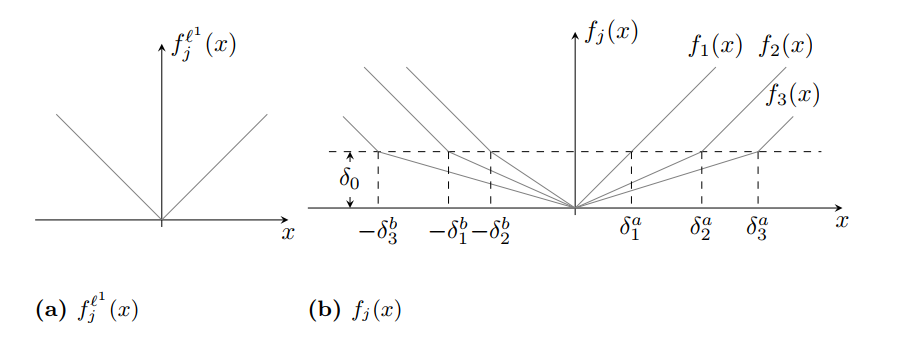
\includegraphics[width = 0.8\linewidth]{bidask.png}
    \caption{Different types of objective functions. (Reference: Cohen et al.~\cite{cohen2020detecting})}
    \label{fig:bidask}
\end{figure}

\section{Conclusion}

The paper on detection of arbitrage by Cohen et al.~\cite{cohen2020detecting} is a very interesting theoretical development for detection of arbitrage opportunities without any underlying model. While several of the assumptions made by the authors (as mentioned before, like availability of only one stock, frictionless market, no missing data) violate the real-life scenario, the method is useful to guide the price determination of options with neural network or machine learning models (that do not themselves rule out arbitrage). 


\printbibliography

\end{document}